% https://2027.msrconf.org/track/msr-2027-data-and-tool-showcase-track

% Data and Tool Showcase Track (maximum 4 pages, plus 1 additional page of
% references)
%
% * a description of the data source,
% * a description of the methodology used to gather the data (including 
%   rovenance and the tool used to create/generate/gather the data, if any),
% * a description of the storage mechanism, including a schema if applicable,
% * if the data has been used by the authors or others, a description of how
%   this was done including references to previously published papers,
% * a description of the originality of the dataset (that is, even if the
%   dataset has been used in a published paper, its complete description must be
%   unpublished) and similar existing datasets (if any),
% * ideas for future research questions that could be answered using the
%   dataset,
% * ideas for further improvements that could be made to the dataset, and
% * any limitations and/or challenges in creating or using the dataset.
%
% If authors developed software to collect, process, or generate the dataset,
% the paper should be accompanied by the source code of the tools, along with
% clear documentation on how to run the tools to recreate the dataset. The tools
% should be open source, accompanied by an appropriate open source license; the
% source code should be citable, i.e., refer to a specific release and have a
%

\documentclass[10pt,conference]{IEEEtran}
\IEEEoverridecommandlockouts
% The preceding line is only needed to identify funding in the first footnote.
% If that is unneeded, please comment it out.

\usepackage{cite}
\usepackage{amsmath,amssymb,amsfonts}
\usepackage{algorithmic}
\usepackage{graphicx}
\usepackage{textcomp}
\usepackage{xcolor}

\usepackage{threeparttable} % recommended IEEEtran package

% extra packages
\usepackage[table]{xcolor}

\usepackage{url}

\usepackage{booktabs}

\usepackage{multirow}
\usepackage{tabularx}

\usepackage{todonotes}
\setuptodonotes{inline}
% NOTE: uncomment to remove todonotes
%\presetkeys{todonotes}{disable}{}

\hyphenation{
  ArKanjo
  kernel Linux
}

\begin{document}

% https://tex.stackexchange.com/questions/458204/ieeetran-document-class-how-to-align-five-authors-properly
\makeatletter
\newcommand{\linebreakand}{%
  \end{@IEEEauthorhalign}
  \hfill\mbox{}\par
  \mbox{}\hfill\begin{@IEEEauthorhalign}
}
\makeatother

% Sub-titles are not captured for https://ieeexplore.ieee.org and should not be
% used
\title{Code Duplication in the Linux Kernel: A Dataset of Discussions, Patches, and Mainline Changes}

% Submissions will undergo single-anonymous peer review.
\author{%
\IEEEauthorblockN{Natália Salvino André}
\IEEEauthorblockA{%
\textit{University of São Paulo (IME-USP)}\\
São Paulo, Brazil \\
natalia.andre@ime.usp.br%
}
\and
\IEEEauthorblockN{Guilherme Ivo}
\IEEEauthorblockA{%
\textit{University of São Paulo (IME-USP)}\\
São Paulo, Brazil \\
guilherme.bozi@usp.br%
}
\and
\IEEEauthorblockN{Gabriel Almeida}
\IEEEauthorblockA{%
\textit{University of São Paulo (ICMC-USP)}\\
São Paulo, Brazil \\
gabrielsousa230@usp.br%
}
\linebreakand
\IEEEauthorblockN{David Tadokoro}
\IEEEauthorblockA{%
\textit{University of São Paulo (IME-USP)}\\
São Paulo, Brazil \\
davidbtadokoro@ime.usp.br%
}
\and
\IEEEauthorblockN{Paulo Meirelles}
\IEEEauthorblockA{%
\textit{University of São Paulo (IME-USP)}\\
São Paulo, Brazil \\
paulormm@ime.usp.br%
}
}

\maketitle

% CRITICAL: Do Not Use Symbols, Special Characters, Footnotes, or Math in Paper
% Title or Abstract.

\begin{abstract}
Code duplication is one of the best-known forms of technical debt. It makes
maintenance more laborious and can lead to inconsistencies, such as a bug being
fixed in one copy but not in the others. In a large, long-lived project like
the Linux kernel, decisions about duplicated code are debated in the open on
mailing lists, where developers propose, question, and reject refactorings,
shared helpers, and copied implementations. These discussions are a rich source
for understanding how this debt is handled in practice, but they are buried
among millions of unrelated emails. We present LKlones, a dataset
of Linux kernel mailing list threads about code duplication, built on top of
the LKML5Ws dataset. Our pipeline groups emails into threads, in which a regex
filter first selects candidate threads and an AI-based classifier sorts each candidate into categories. Out of 3.7 million threads from 206 mailing lists, the classifier
labels more than 186,000 threads as related to code duplication, and over
33,000 of them are linked to commits that reached the mainline kernel. Each
thread includes its messages, its category with a confidence score, and its
links to commits.
\end{abstract}

\begin{IEEEkeywords}
Linux kernel, Code Duplication, Mailing Lists
\end{IEEEkeywords}

\section{Introduction}

Code duplication is one of the best-known forms of technical debt, being the
first entry in Fowler's catalog of code smells~\cite{fowler1999refactoring}. This debt can be observed in large and
relevant software projects, such as the Linux kernel, a widely known project
maintained for over three decades by a large community. Despite its careful
architecture, it still contains duplicated code, including large clones of
files and directories~\cite{kumar2016bigclones}. Since its code and development history are publicly available in large volume, exploring how the kernel deals with this form of technical debt can offer valuable insights into how developers manage this debt in practice.

Prior work has explored this history only partially. Wang and Godfrey searched the Linux commit
history for the phrase \textit{``duplicated code''} to build a dataset of intentional
clone refactoring~\cite{wang2014intentional}. Their search relies on a single
phrase and sees only merged changes, missing
rejected and the review discussions around the topic. These discussions take place on the kernel mailing lists~\cite{linux_process_mailinglist}, making them a natural source for closing this gap. Mining them, however, is not straightforward, since duplication is rarely mentioned in developer communication. In commit messages, for instance, only 348 of the 28,538 analyzed by Wang and Godfrey mention duplicated
code~\cite{wang2014intentional}. Finding the relevant threads among millions of emails therefore requires a systematic selection process.

In this paper, we present \textsc{LKlone}, a dataset of Linux kernel
mailing-list threads about code duplication. It builds on \textsc{LKML5Ws}~\cite{passos2026lkml5ws}, a dataset with almost 30 million emails exchanged on the Linux kernel mailing lists. A pipeline builds the dataset, starting with the reconstruction of the threads of each list, since the discussion around a patch involves several emails. It then identifies the threads about duplication by combining a regular-expression filter with an AI-based classification. Finally, it links these threads to the commits that reached the
mainline kernel.

From 23,8 million of emails, 3.7 million threads in 206 mailing lists, we classify 186,432 threads
as being about code duplication, providing the content of each thread with the
whole discussion around it. Of these threads, 33,209 are linked to
mainline commits. This dataset supports studies of how kernel developers handle
duplication, bringing complete discussions on the topic, including patches that maintainers rejected or ignored.


\section{Data collection and processing}


% showcase: dada o subconjunto de clone refactoring, usar o jev para encontrar os motivos. Aplicações relacionadas aos trabalhos ja realizados (foco na comunidade de divida tecnica) que se beneficiariam do nosso dataset
% background: clones (conceito, se der, falar dos tipos t1-t4), mailing lists, patch (esclarecer que ha codigo aqui), thread, commit mainline

Figure~\ref{fig:pipeline} summarizes the five-step pipeline that builds
\textsc{LKlone}. Once the threads are assembled, no step removes data, and each step
only adds columns to the dataset, so users can apply their own filters.

\subsection{Collect}

The input is \textsc{LKML5Ws}~\cite{passos2026lkml5ws}, a dataset of the
mailing lists hosted on \texttt{lore.kernel.org} with one email per row. \textsc{LKML5Ws}
also covers lists unrelated to the kernel source code, such as the Git mailing
list. To keep only kernel development, we accept a list when it is the official
list of a subsystem in the kernel \texttt{MAINTAINERS} file that covers files of
the repository, in at least one release between v2.6.30 and v7.2. This criterion
keeps 206 of the 353 lists of \textsc{LKML5Ws} in our dataset.

\subsection{Thread Construction}

A single email rarely tells the whole story of a patch. Since we want
the complete discussion, we group the emails into threads. Emails are linked to their parents through the \texttt{In-Reply-To} header and
grouped into threads with a union-find structure. When the parent is missing
from \textsc{LKML5Ws}, the last identifier in the \texttt{References} header is used
instead. Messages within a thread are kept in chronological order. This is the
only step that removes data, as we discard pull requests (e.g., \texttt{[GIT PULL]}),
which only summarize patches discussed in other threads, and messages sent by
bots, such as syzbot. The result is 3.7 million threads
built from 23.8 million emails.

Since duplication is rarely discussed, a regular-expression pre-filter then
flags the threads that may be about it. We built the regular expressions from a vocabulary analysis, in which two
reviewers manually inspected a sample of threads and identified the terms
that developers use when discussing duplication, such as \textit{duplicat*},
\textit{dedup*}, \textit{redundant*}, \textit{copy-paste}, and phrases like
``move into a common helper''. The same analysis revealed recurring false
positives, such as ``redundant null check'' and ``duplicate include'', which
we added as exclusions. Quoted text is ignored, so that each passage only counts
in the message where it was written. The pre-filter flags 373,264 candidate
threads (\texttt{is\_duplication\_candidate}), and only these receive the
concatenated text of their messages (\texttt{thread\_content}).

\subsection{Classify}

The pre-filter favors recall, so many candidates are not actually about
duplication. To separate them, a large language model (LLM) decides whether
each candidate thread is related to duplication. In preliminary tests, the
model performed poorly when asked yes-or-no questions directly. We therefore
guide it with five categories that describe what we consider related to
duplication. A thread is \textit{clone refactoring} when a patch consolidates
existing copies into a single place, \textit{preventive reuse} when a patch
avoids writing a copy by reusing or sharing code, and \textit{clone and reuse}
when both occur in the same thread. It is \textit{duplication discussion} when
participants discuss duplication but no patch acts on it, and
\textit{not duplication} otherwise. The categories serve only as guidance, and
the first four are mapped to \textit{yes}, while the last is mapped to
\textit{no}.

We use Jev~\cite{typesafe_jev}, version 1.13.0, selected after comparing it with other
LLMs. We frame the task as a choice question, in which Jev picks one of the five
categories for each thread. Instead of free-form text, Jev returns the
probability of each category, which keeps the output structured and
reproducible across runs. The
chosen category and its probability are stored in \texttt{category} and
\texttt{category\_confidence}, letting users set their own confidence threshold.
Threads longer than the model context are truncated,
keeping the first message and the passages around the pre-filter terms.

To evaluate the classifier, two authors independently labeled 313
threads sampled from four lists, reaching 87.9\% agreement (Cohen's
$\kappa = 0.82$) and resolving disagreements by consensus.
On the binary decision, Jev reaches 84.7\% accuracy, with 95.3\% recall and
70.3\% precision for threads about duplication. The classifier thus rarely misses
relevant threads, and users who need higher precision can rely on
\texttt{category\_confidence}. In total, 186,432 threads are classified as being
about duplication.

\subsection{Match}

We then link the threads to the commits that reached the mainline kernel. For
each commit in the mainline history, we search for the email that introduced
it. A commit is linked to an email with status
\texttt{LINK} when its \texttt{Link:} trailer cites the email Message-ID.
Otherwise, it is linked with status \texttt{EXACT} when the author email (or its
hash) and the author date match the sender and date of a patch email, or with
status \texttt{AMBIGUOUS} when more than one email matches, in which case all
candidates are kept. These links are stored in \texttt{commit\_matches}. Overall,
33,209 threads about duplication are linked to 84,964 distinct commits.

\subsection{Anonymize and Publish}

We use the anonymized release of \textsc{LKML5Ws}, in which the names and
email addresses of participants are already replaced by SHA-1 hashes, but
Message-IDs are kept in clear text. Since a Message-ID often embeds the
sender's address or host name, we complete this anonymization by applying the
same hash to every Message-ID in the output. Each thread is identified by the hash of its first
message (\texttt{thread\_id}). The resulting dataset is stored in Apache Parquet, with one
row per thread and the columns described in Table~\ref{tab:dataset-schema},
and is publicly available on Zenodo\todo{colocar Zenodo DOI}.

\begin{figure*}[t]
  \centering
  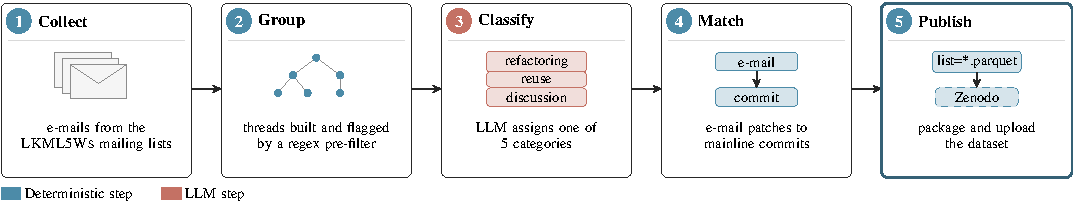
\includegraphics[width=\textwidth]{figures/pipeline.pdf}
  \caption{Overview of the dataset construction pipeline.}
  \label{fig:pipeline}
\end{figure*}

\begin{figure}[ht]
  \centering
  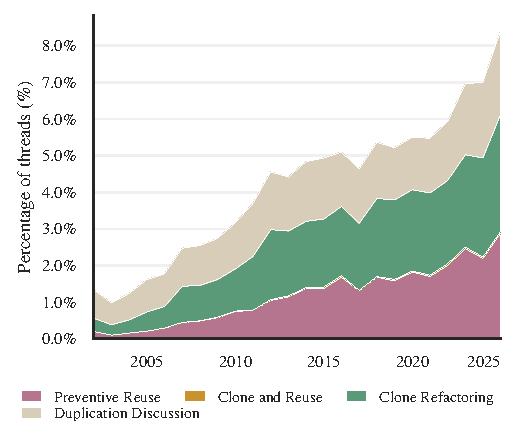
\includegraphics[width=\columnwidth]{figures/yearly_area.pdf}%
  \vspace{-10pt}
  \caption{Yearly proportion of threads across duplication-related categories. Stacked areas represent the four duplication-related categories, showing their respective proportions of all threads analyzed each year.}
  \label{fig:yearlyarea}
\end{figure}

\begin{table}[t]
  \centering
  \caption{Parquet dataset schema. Each row represents a mailing-list thread.}
  \label{tab:dataset-schema}
  \footnotesize
  \begin{tabularx}{\columnwidth}{@{} l l X @{}}
    \toprule
    \textbf{Column} & \textbf{Type} & \textbf{Description} \\
    \midrule
    \texttt{thread\_id} & String & Unique identifier of the thread. \\
    \texttt{list} & String & Mailing list from which the thread originated. \\
    \texttt{n\_messages} & Int64 & Number of messages in the thread. \\
    \texttt{message\_ids} & List[String] & Message identifiers in chronological order. \\
    \texttt{date} & Timestamp & Date of the first message. \\
    \texttt{subject} & String & Subject of the first message. \\
    % is\_duplication\_candidate
    \texttt{dup\_candidate} & Boolean & Indicates whether the thread matches the regex pre-filter. \\
    \texttt{thread\_content} & String & Concatenated content of the messages. \\
    \texttt{category} & String & Classification assigned to the thread. \\
    \texttt{category\_confidence} & Double & Confidence score of the classification. \\
    \texttt{commit\_matches} & List[Struct] & Commits associated with messages in the thread. \\
    \midrule
    \multicolumn{3}{@{}l}{\textit{Fields of \texttt{commit\_matches}}} \\
    \addlinespace[2pt]
    \texttt{message\_id} & String & Message associated with the commit. \\
    \texttt{commit\_hash} & String & Hash of the mainline commit. \\
    \texttt{status} & String & Matching method: \texttt{LINK}, \texttt{EXACT}, or \texttt{AMBIGUOUS}. \\
    % candidate\_message\_ids
    \texttt{ambiguous\_ids} & List[String] & Candidate messages when the match is ambiguous. \\
    \bottomrule
  \end{tabularx}
\end{table}

\bibliographystyle{IEEEtran}
\bibliography{IEEEabrv,references}

\end{document}
% dataset collection and processing